\subsection{INTERFACE}

A interface \textit{web} é responsável pela interação do usuário final com a aplicação. Portanto, implementaram-se funcionalidades que possibilitam a configuração das restrições e características das grades horárias a serem geradas, além de mostrar ou exportar tais grades após a geração.

Para o desenvolvimento deste componente, optou-se pelo framework \textit{Vue.js}, devido à riqueza de seu ecossistema de desenvolvimento \textit{frontend} e familiaridade do graduando com este. Complementando este framework, utilizou-se também o \textit{Vuetify.js}, a fim de facilitar e padronizar o design da aplicação.

A \autoref{fig:diagrama-uc} mostra os casos de uso que a interface \textit{web} é responsável por disponibilizar:

\begin{figure}[!htb]
	\centering
	\caption{Diagrama de Casos de Uso}
	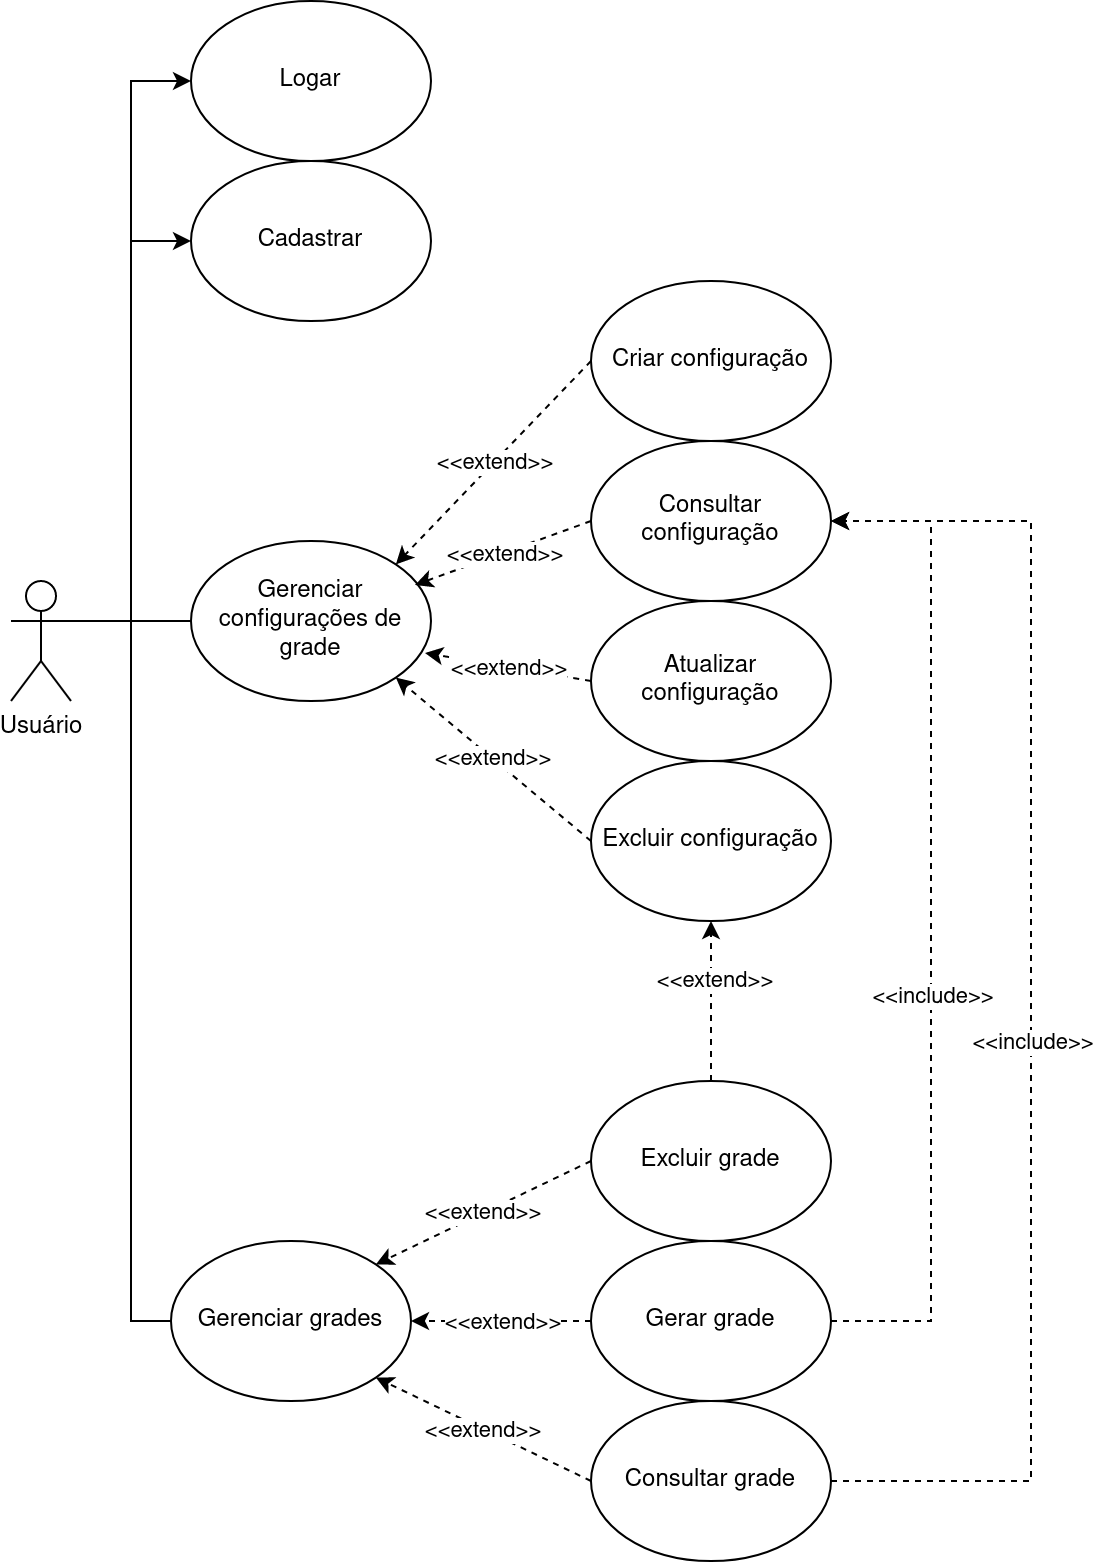
\includegraphics[width=0.65\textwidth]{./dados/figuras/diagrama_uc}
	\fonte{Autor}
	\label{fig:diagrama-uc}
\end{figure}
\newpage

A \autoref{fig:tela-configuracoes} mostra a tela de listagem de configurações de grade. Como comentado anteriormente, alguns dos casos de uso da aplicação envolvem o gerenciamento de configurações de grades horárias, as quais são listadas nessa tela.

\begin{figure}[!htb]
	\centering
	\caption{Tela - Listagem de Configurações de Grade}
	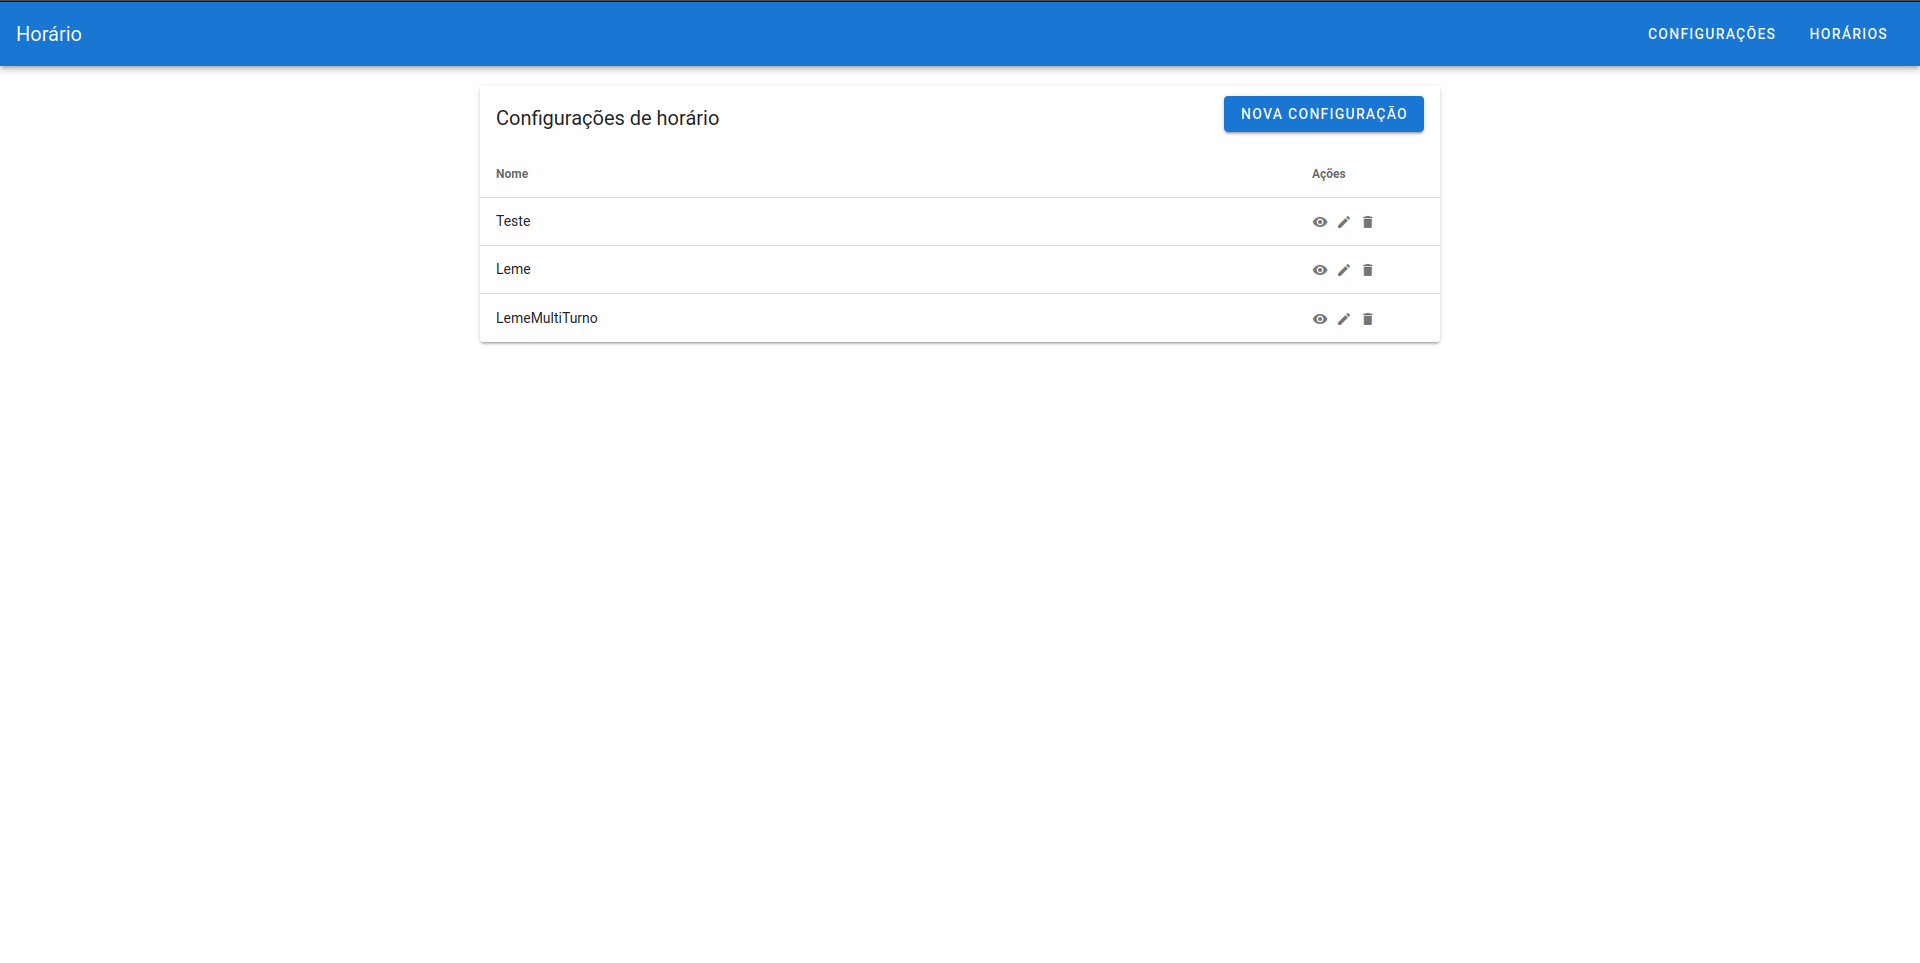
\includegraphics[width=0.8\textwidth]{./dados/figuras/tela_configuracoes}
	\fonte{Autor}
	\label{fig:tela-configuracoes}
\end{figure}
\pagebreak

A tela mostrada na \autoref{fig:tela-estrutura1} é responsável por permitir que o usuário cadastre os professores da escola. Nessa tela é possível notar que a aplicação foi estruturada seguindo uma noção de etapas de configuração até a geração da grade horária final. No topo da tela, a etapa ``Estrutura da Escola'' encontra-se selecionada.

\begin{figure}[!htb]
	\centering
	\caption{Tela - Estrutura da Escola - Professores}
	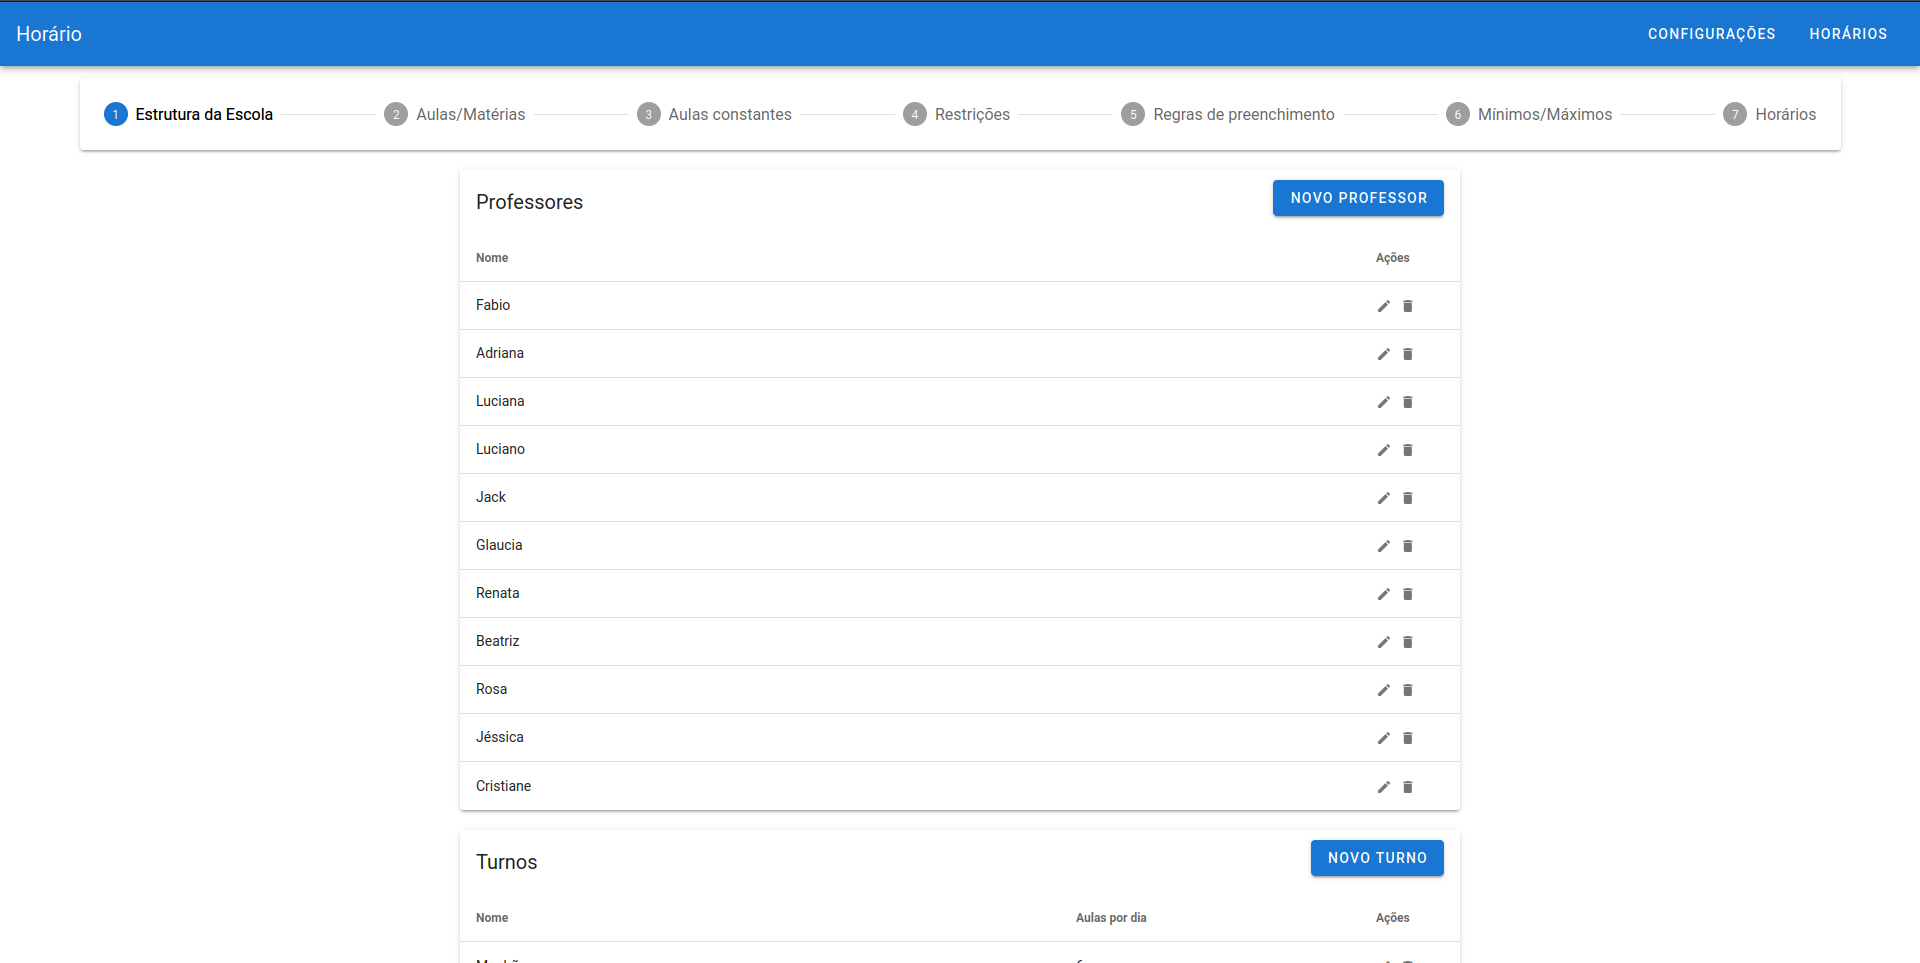
\includegraphics[width=0.8\textwidth]{./dados/figuras/tela_estrutura1}
	\fonte{Autor}
	\label{fig:tela-estrutura1}
\end{figure}
\newpage

Na \autoref{fig:tela-estrutura2}, tem-se a continuação da tela de estrutura da escola, mostrada na \autoref{fig:tela-estrutura1}. Esta parte da tela é responsável pela configuração das turmas e turnos da escola.

\begin{figure}[!htb]
	\centering
	\caption{Tela - Estrutura da Escola - Turmas e Turnos}
	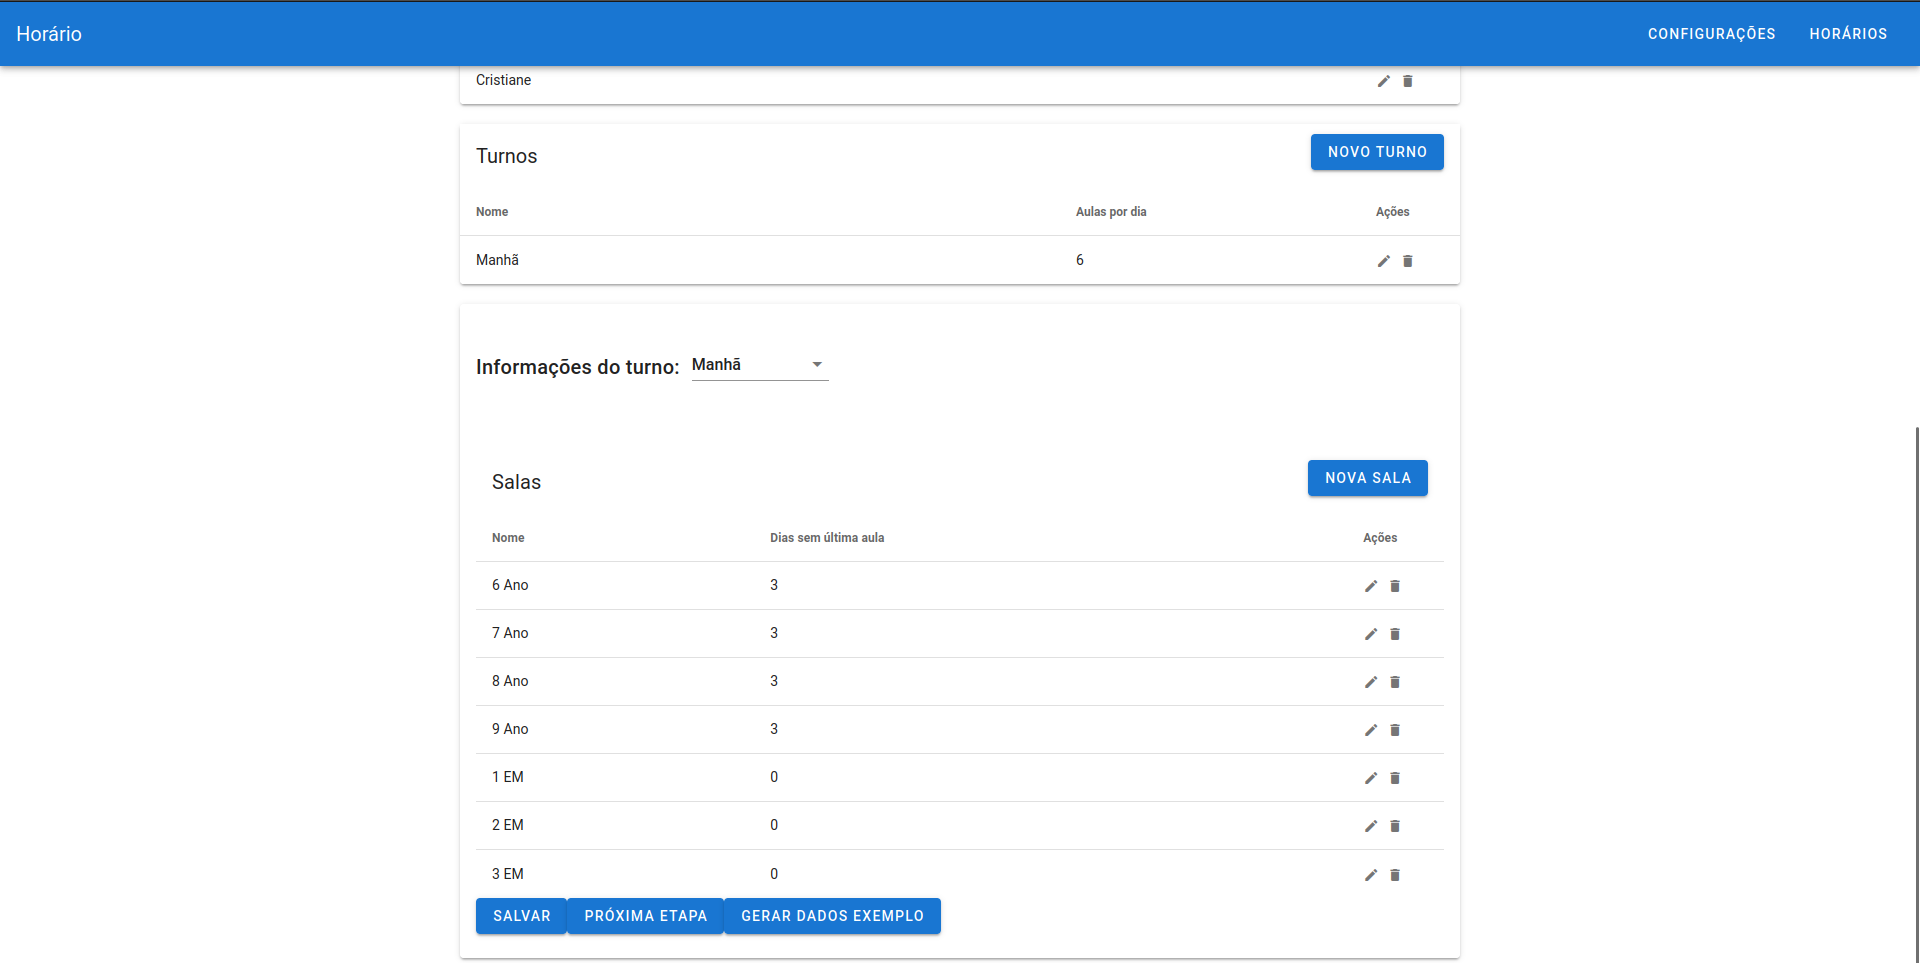
\includegraphics[width=0.8\textwidth]{./dados/figuras/tela_estrutura2}
	\fonte{Autor}
	\label{fig:tela-estrutura2}
\end{figure}

Na tela da \autoref{fig:tela-aulas}, o usuário pode realizar a configuração de número de aulas que cada professor deve ministrar em cada sala, informação fundamental para a geração das grades horárias.

\begin{figure}[!htb]
	\centering
	\caption{Tela - Aulas por professor}
	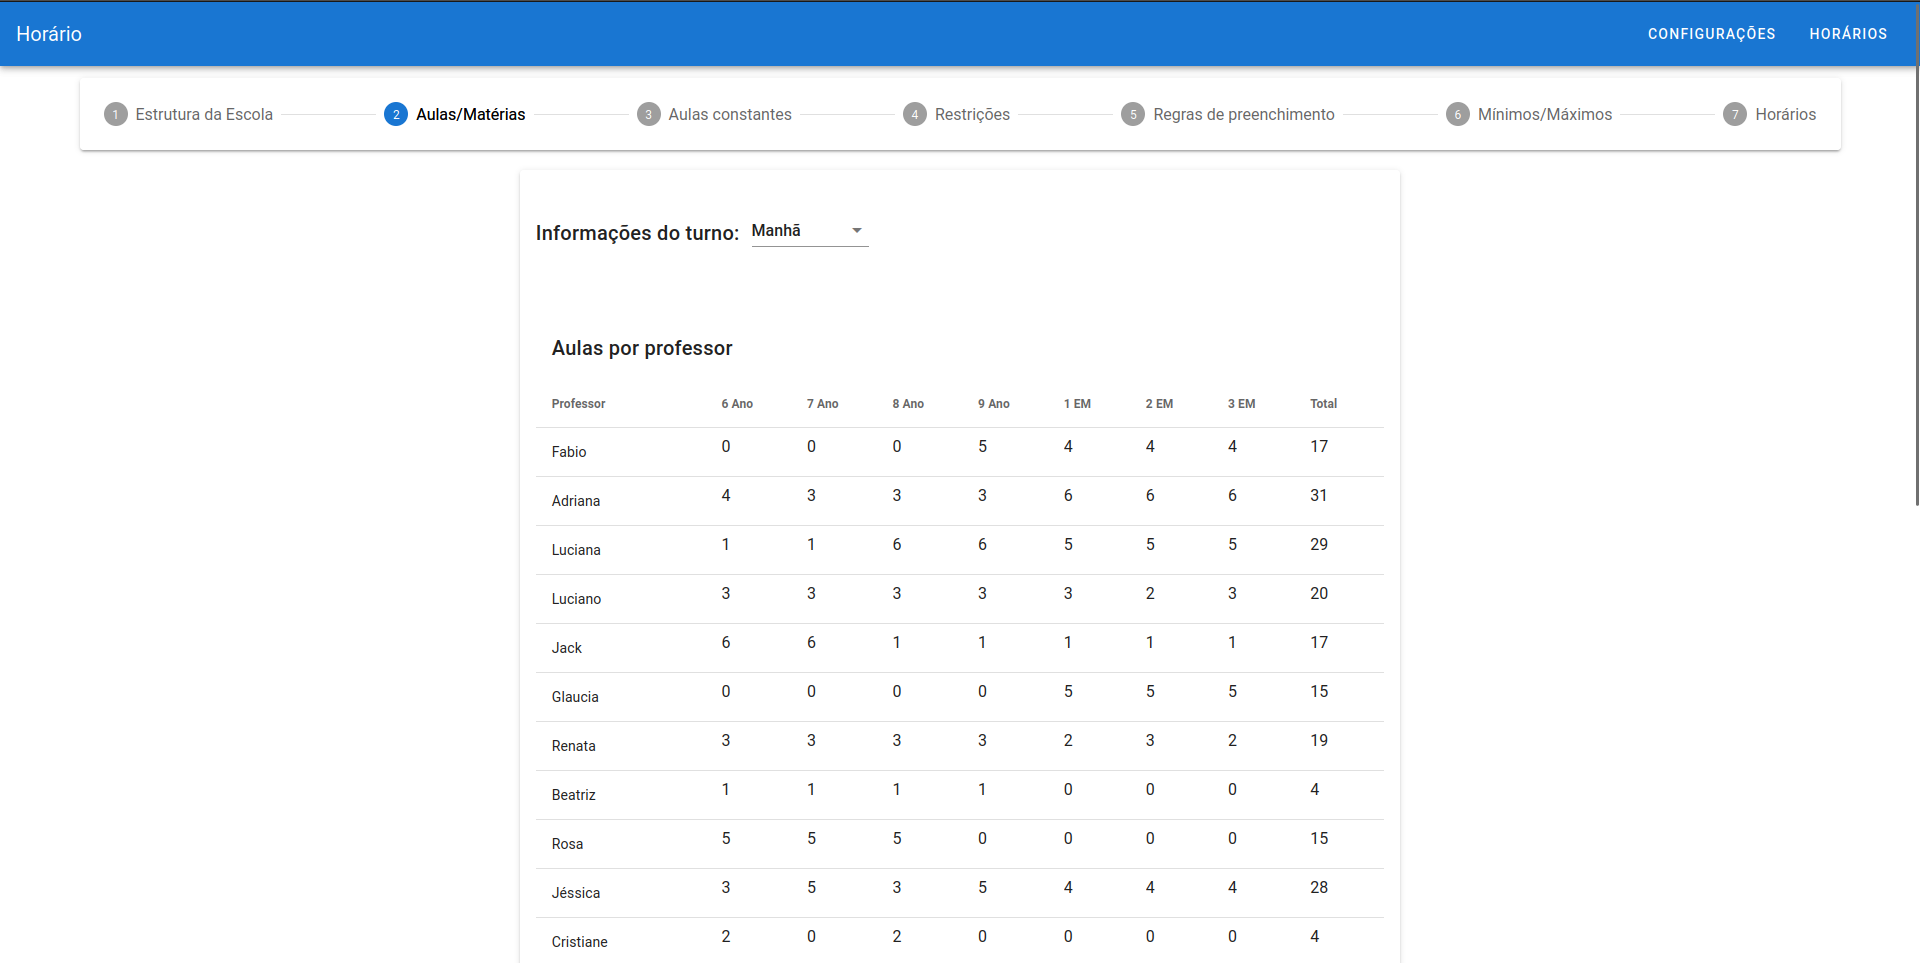
\includegraphics[width=0.8\textwidth]{./dados/figuras/tela_aulas}
	\fonte{Autor}
	\label{fig:tela-aulas}
\end{figure}
\newpage

A tela da \autoref{fig:tela-restricoes} é responsável pela configuração das restrições e preferências. Nesta, o usuário pode configurar horários na grade que devem ser evitados ou proibidos para determinado docente.

\begin{figure}[!htb]
	\centering
	\caption{Tela - Restrições e Preferências}
	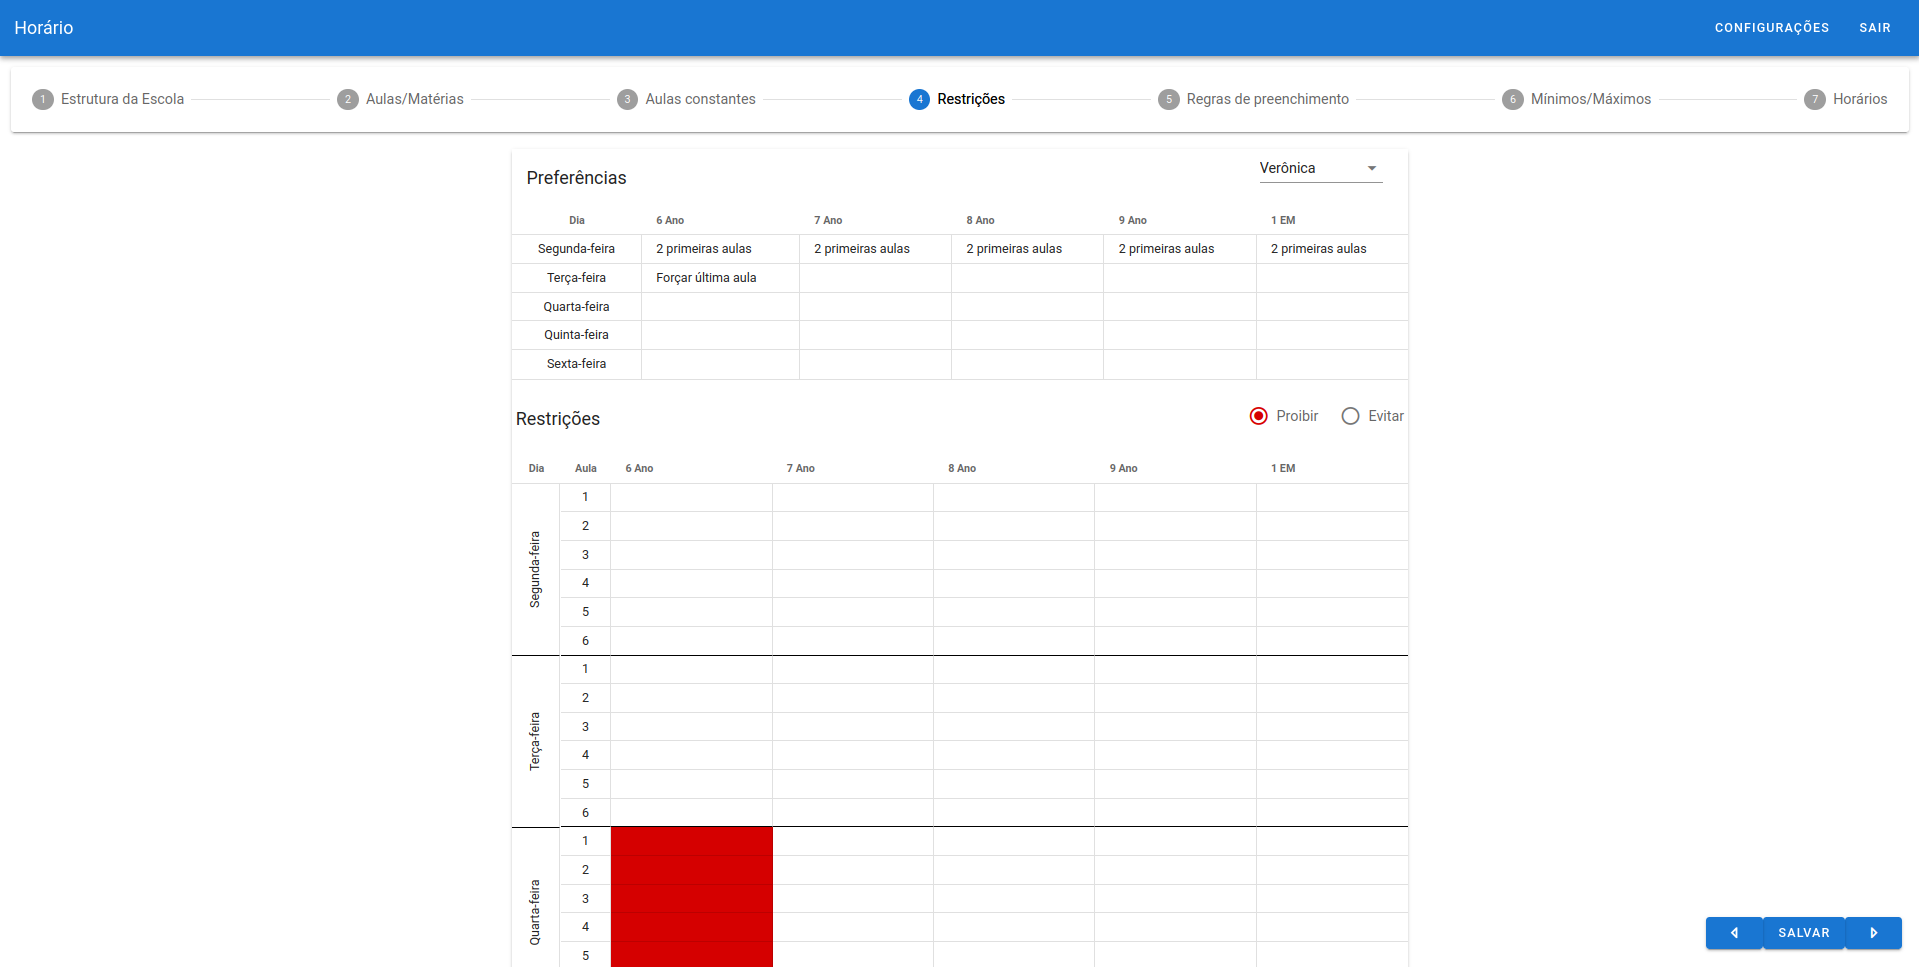
\includegraphics[width=0.8\textwidth]{./dados/figuras/restricoes_nova}
	\fonte{Autor}
	\label{fig:tela-restricoes}
\end{figure}

Já a tela da \autoref{fig:tela-regioes} possibilita a configuração das regiões e grupos de alinhamento:

\begin{figure}[!htb]
	\centering
	\caption{Tela - Regiões e Grupos de Alinhamento}
	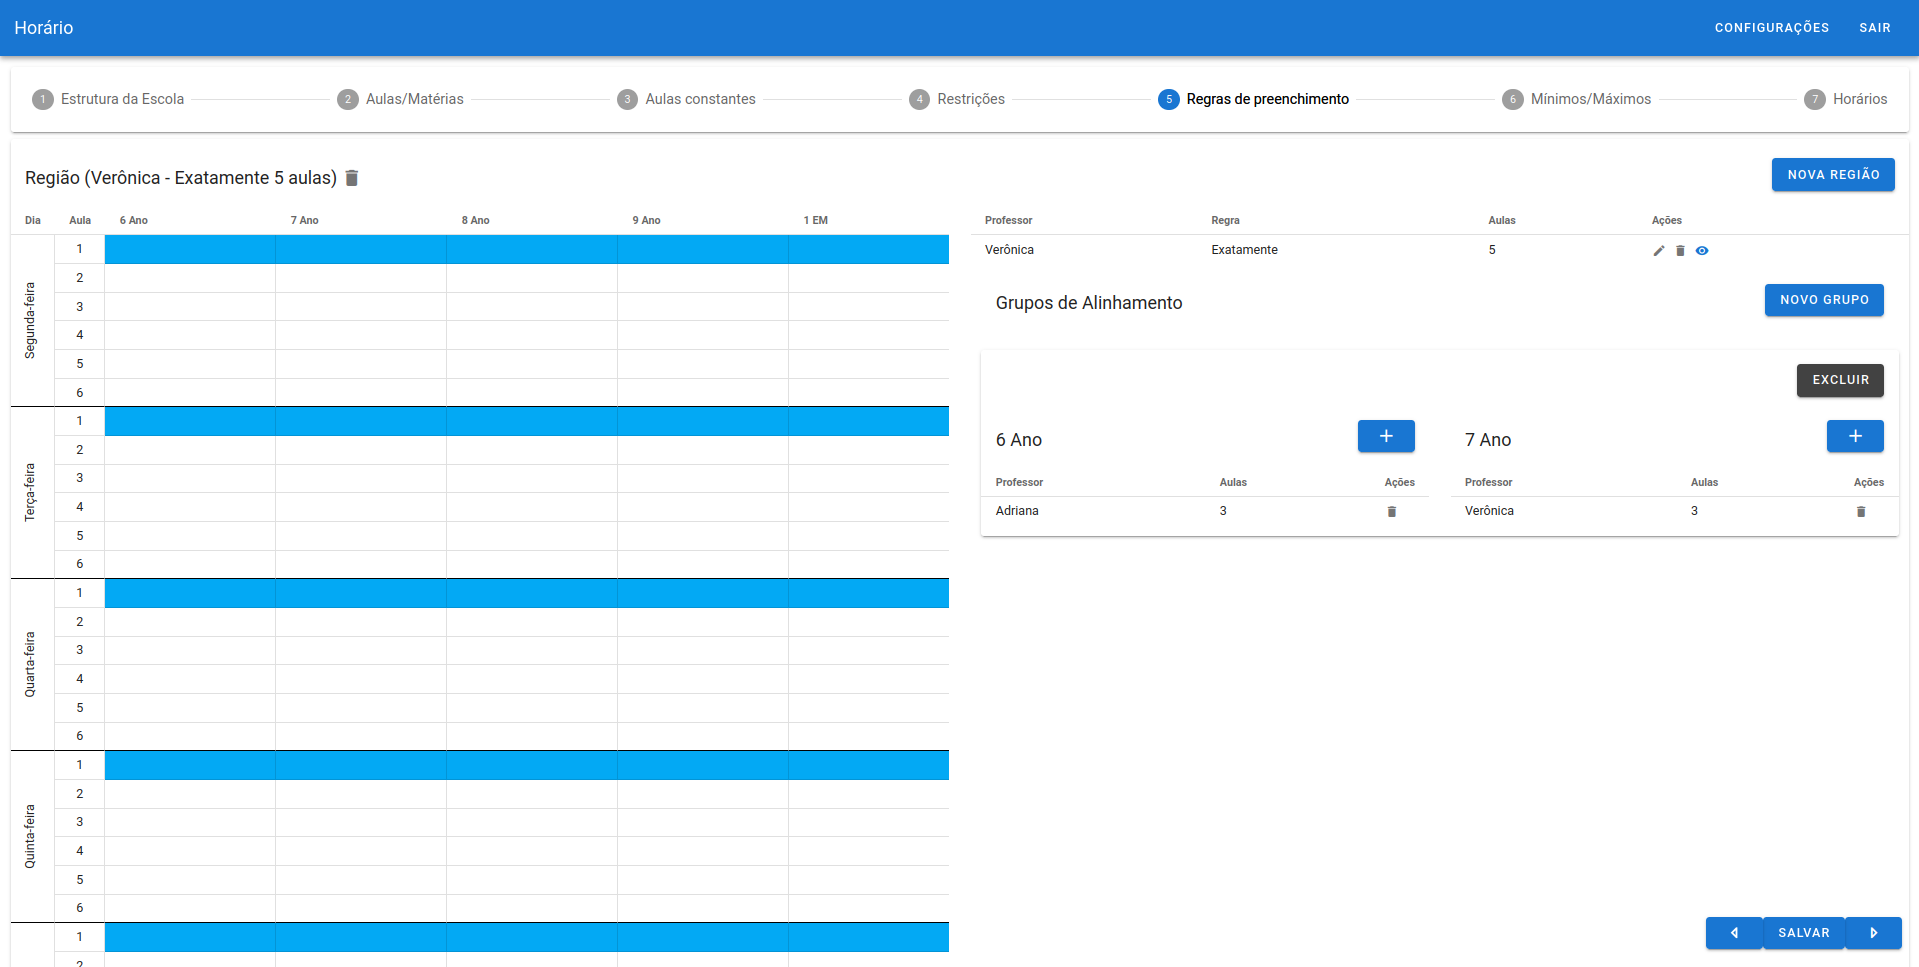
\includegraphics[width=0.8\textwidth]{./dados/figuras/tela_regioes}
	\fonte{Autor}
	\label{fig:tela-regioes}
\end{figure}

A última tela relacionada a configurações pode ser vista na \autoref{fig:tela-minimos-maximos}, e permite a definição de quantidade mínimas e máximas de aulas para cada professor em cada dia da grade horária:

\begin{figure}[!htb]
	\centering
	\caption{Tela - Mínimos e Máximos}
	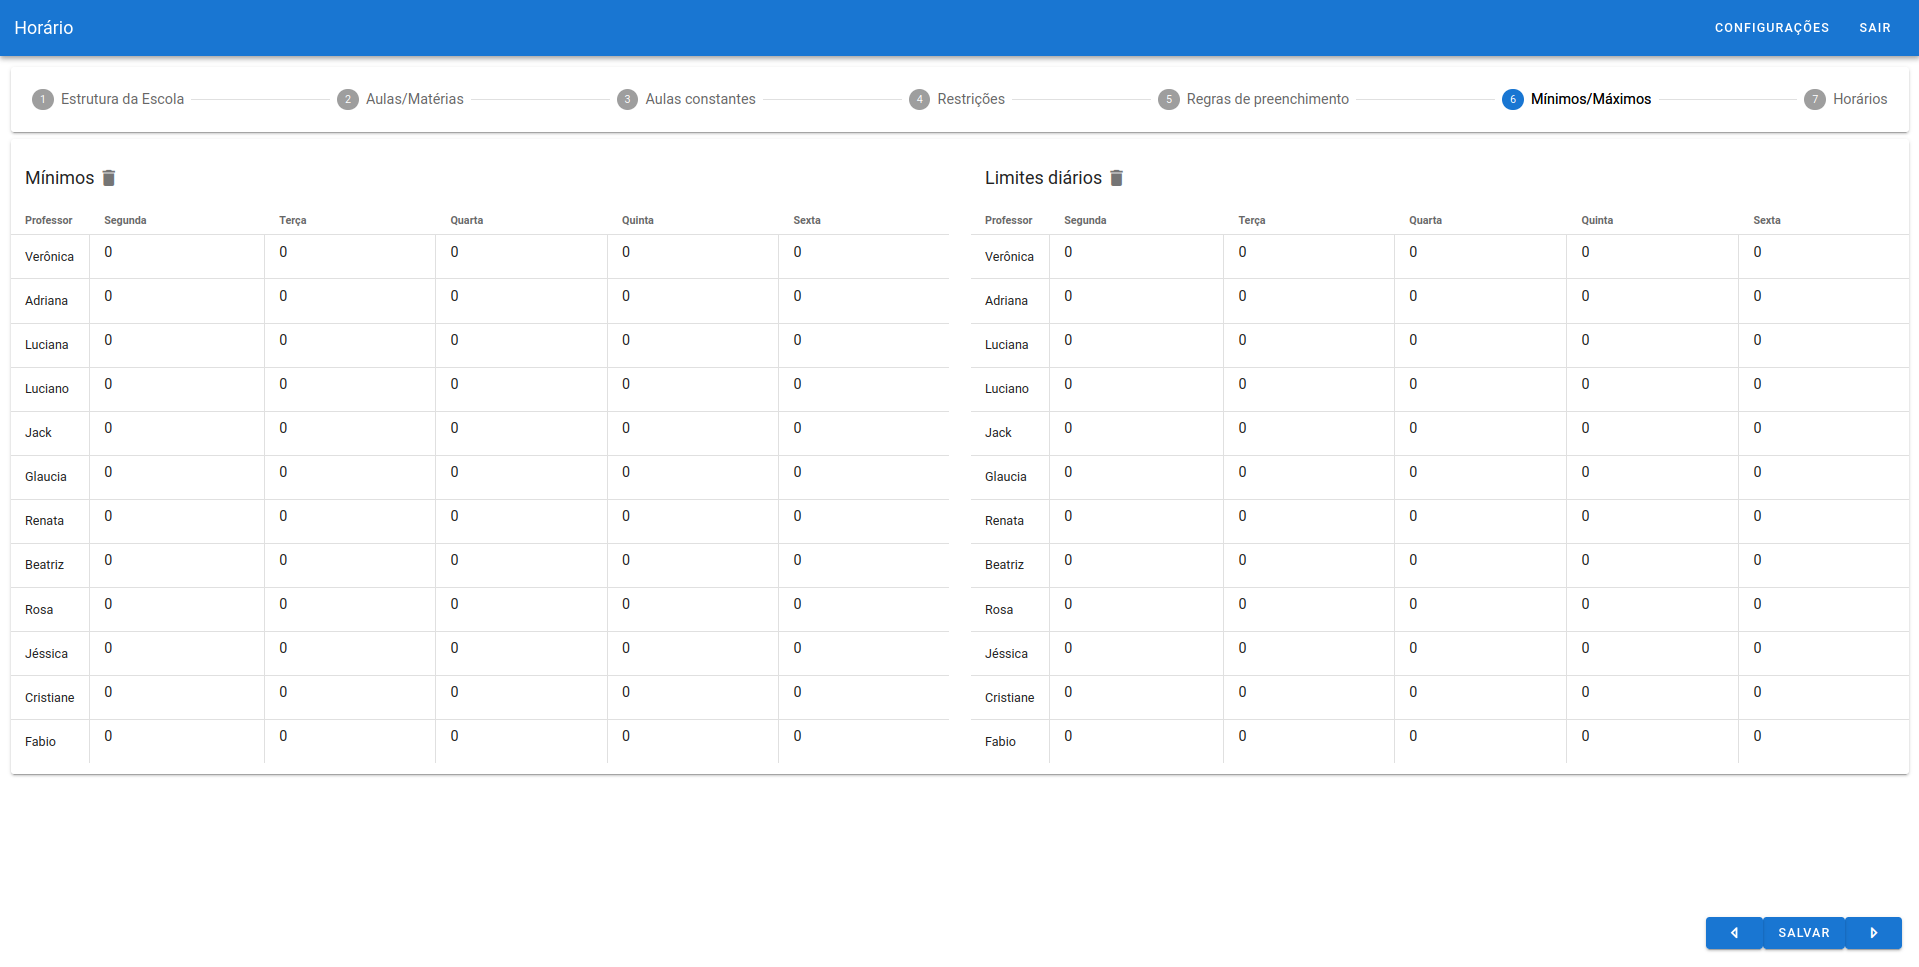
\includegraphics[width=0.8\textwidth]{./dados/figuras/tela_minimos_maximos}
	\fonte{Autor}
	\label{fig:tela-minimos-maximos}
\end{figure}

A etapa final no fluxo da aplicação é representada pela tela da \autoref{fig:tela-horarios}. Nesta, o usuário pode requisitar a geração da grade horária utilizando as configurações realizadas nas etapas anteriores, e acessar as grades geradas anteriormente.

\begin{figure}[!htb]
	\centering
	\caption{Tela - Horários}
	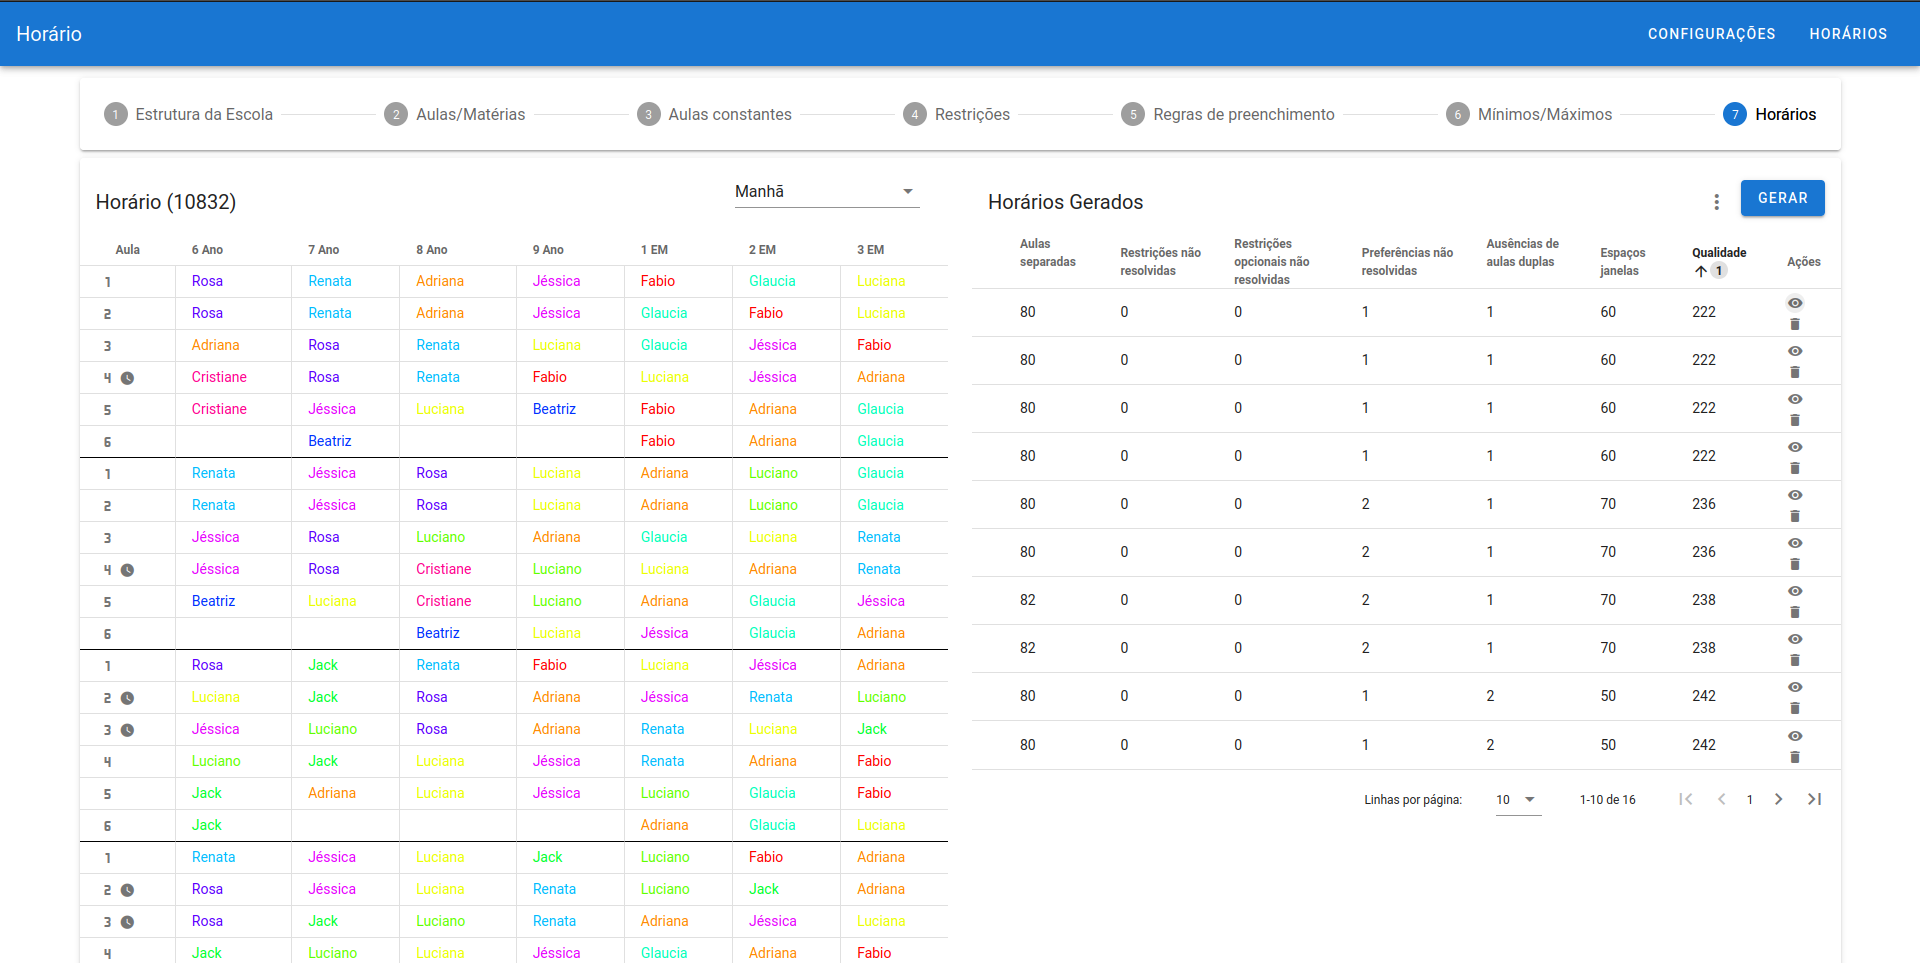
\includegraphics[width=0.8\textwidth]{./dados/figuras/tela_horarios}
	\fonte{Autor}
	\label{fig:tela-horarios}
\end{figure}
\newpage